\documentclass[UTF8]{ctexart}
\usepackage[colorlinks=true]{hyperref}
\usepackage[a4paper,scale=0.8,centering]{geometry}
\usepackage{amsmath,amssymb,mathtools}
\usepackage{xcolor}
\usepackage{longtable}
\usepackage{listings}
\lstset{
        columns=flexible,
        basicstyle=\ttfamily,
        commentstyle=\color{green}\rmfamily\itshape,
        backgroundcolor=\color{gray!20}}

\usepackage{tikz}

\usetikzlibrary{intersections,
                positioning,
                petri,
                backgrounds,
                fit,
                decorations.pathmorphing,
                arrows,
                arrows.meta,
                bending,
                calc,
                intersections,
                through,
                backgrounds,
                shapes.geometric,
                quotes,
                matrix,
                trees,
                shapes.symbols,
                graphs,
                math,
                patterns,
                external}

\title{Tikz 学习笔记}
\author{}



\begin{document}

\ttfamily

\setlength\parskip{0.3cm}

\maketitle

\tableofcontents

\newpage

\section{三类例子}

\subsection{单位圆与三角函数线}

本小节展示的代码绘制下面的图形
\begin{figure}[h]
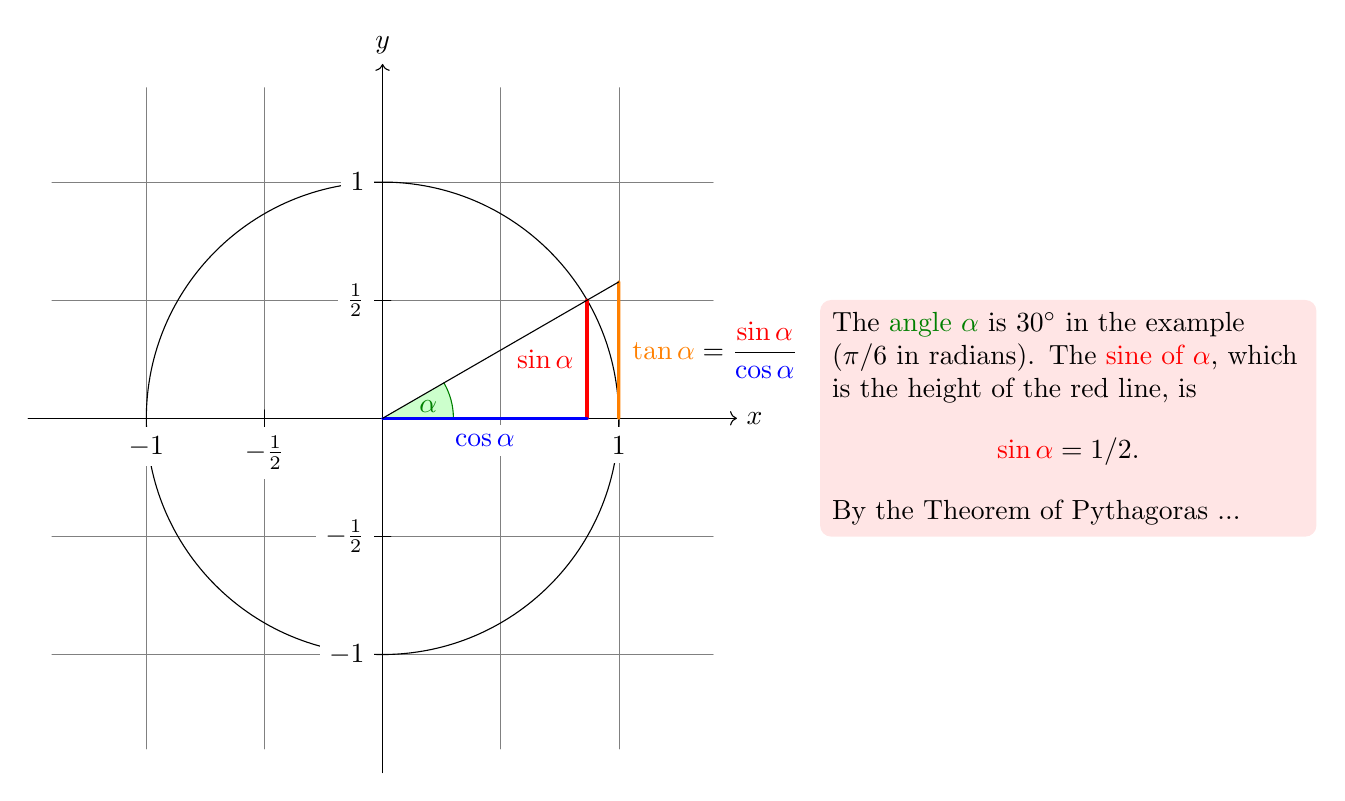
\begin{tikzpicture}
[scale=3,line cap=round,axes/.style=,important line/.style={very thick},
information text/.style={rounded corners,fill=red!10,inner sep=1ex}]
% Colors
\colorlet{anglecolor}{green!50!black}
\colorlet{sincolor}{red}
\colorlet{tancolor}{orange!80!black}
\colorlet{coscolor}{blue}
% The graphic
\draw[help lines,step=0.5cm] (-1.4,-1.4) grid (1.4,1.4);
\draw (0,0) circle [radius=1cm];
\begin{scope}
\draw[->] (-1.5,0) -- (1.5,0) node[right] {$x$} coordinate(x axis);
\draw[->] (0,-1.5) -- (0,1.5) node[above] {$y$} coordinate(y axis);
\foreach \x/\xtext in {-1, -.5/-\frac{1}{2}, 1}
\draw[xshift=\x cm] (0pt,1pt) -- (0pt,-1pt) node[below,fill=white] {$\xtext$};
\foreach \y/\ytext in {-1, -.5/-\frac{1}{2}, .5/\frac{1}{2}, 1}
\draw[yshift=\y cm] (1pt,0pt) -- (-1pt,0pt) node[left,fill=white] {$\ytext$};
\end{scope}
\filldraw[fill=green!20,draw=anglecolor] (0,0) -- (3mm,0pt)
arc [start angle=0, end angle=30, radius=3mm];
\draw (15:2mm) node[anglecolor] {$\alpha$};
\draw[important line,sincolor]
(30:1cm) -- node[left=1pt,fill=white] {$\sin \alpha$} (30:1cm |- x axis);
\draw[important line,coscolor]
(30:1cm |- x axis) -- node[below=2pt,fill=white] {$\cos \alpha$} (0,0);
\path [name path=upward line] (1,0) -- (1,1);
\path [name path=sloped line] (0,0) -- (30:1.5cm);
\draw [name intersections={of=upward line and sloped line, by=t}]
[very thick,orange] (1,0) -- node [right=1pt,fill=white]
{$\displaystyle \tan \alpha \color{black}=
\frac{{\color{red}\sin \alpha}}{\color{blue}\cos \alpha}$} (t);
\draw (0,0) -- (t);
\draw[xshift=1.85cm]
node[right,text width=6cm,information text]
{
The {\color{anglecolor} angle $\alpha$} is $30^\circ$ in the
example ($\pi/6$ in radians). The {\color{sincolor}sine of
$\alpha$}, which is the height of the red line, is
\[
{\color{sincolor} \sin \alpha} = 1/2.
\]
By the Theorem of Pythagoras ...
};
\end{tikzpicture}
\end{figure}

\begin{lstlisting}[name=example-1,numbers=left,    numberstyle=\footnotesize]
\begin{tikzpicture}
[scale=3,line cap=round,
% Styles
axes/.style=,
important line/.style={very thick},
information text/.style={rounded corners,
                              fill=red!10,inner sep=1ex}]
% Colors
\colorlet{anglecolor}{green!50!black}
\colorlet{sincolor}{red}
\colorlet{tancolor}{orange!80!black}
\colorlet{coscolor}{blue}
\end{lstlisting}

1行,开启tikzpicture环境。

2行,scale=3,缩放比例为3。line cap=round,线的端头采用圆形(rect为方形,butt为无头)。

4行,axes 采用默认样式。

5行,定义important line的样式,只要求线宽为very thick。

6行,定义information text的样式,圆角边框,颜色为red!10,文字与文字背景边界距离为1ex。

9行,命令 \verb!\colorlet! 定义颜色green!50!black的名称为anglecolor,可以用此名称引用该颜色。10、11、12行类似。

\begin{lstlisting}[name=example-1,numbers=left,    numberstyle=\footnotesize]
% The graphic
\draw[help lines,step=0.5cm] (-1.4,-1.4) grid (1.4,1.4);
\draw (0,0) circle [radius=1cm];
\begin{scope}[axes]
\draw[->] (-1.5,0) -- (1.5,0) node[right] {$x$} 
            coordinate(x axis);
\draw[->] (0,-1.5) -- (0,1.5) node[above] {$y$} 
            coordinate(y axis);
\foreach \x/\xtext in {-1, -.5/-\frac{1}{2}, 1}
\draw[xshift=\x cm] (0pt,1pt) -- (0pt,-1pt) 
                     node[below,fill=white] {$\xtext$};
\foreach \y/\ytext in {-1, -.5/-\frac{1}{2}, .5/\frac{1}{2}, 1}
\draw[yshift=\y cm] (1pt,0pt) -- (-1pt,0pt) 
                     node[left,fill=white] {$\ytext$};
\end{scope}
\end{lstlisting}

14行,\verb!\draw!命令开始绘图,grid 是网格命令,采用help lines的样式,步长step=0.5cm,以点(-1.4,-1.4)到(1.4,1.4)为对角线。

15行,画圆,圆心为(0,0),半径为radius=1cm。

16行,开启scope环境,即在整个大图中再绘制一个局部图。

17行,从(-1.5,0)到(1.5,0)画线段,选项[->]为线段末端添加箭头;点(1.5,0)后的node命令为该点添加标签,选项[right]指示标签在点的右侧,标签是 \LaTeX 符号$x$。

21行,\verb!\foreach!命令指示对数组中的每个元素进行后面的操作。\verb!\x/\xtext!
表示数组元素可以是\verb!\x!形式的或\verb!\x/\xtext!形式的;同一个元素位置上用符号/并列两种形式时,该元素可用两种形式之一引用。数组 \{1,...,10\}是公差为1的等差数列,数组\{1,1.5,,...,10\}是公差为前两项之差0.5的等差数列。

22行,是21行的\verb!\foreach!命令指向的操作。选项 \verb![xshift=\x cm]!指示将后面绘制的线段沿着x轴平移 \verb!\x cm!。

23行,node命令为22行的点(0pt,-1pt)加标签,标签用 \verb!$\xtext$!形式。选项[below,fill=white]表示标签在点下方,标签背景为白色。

27行,结束scope环境。

\begin{lstlisting}[name=example-1,numbers=left,    numberstyle=\footnotesize]
\filldraw[fill=green!20,draw=anglecolor] (0,0) -- (3mm,0pt)
arc [start angle=0, end angle=30, radius=3mm];
\draw (15:2mm) node[anglecolor] {$\alpha$};
\draw[important line,sincolor]
      (30:1cm) -- node[left=1pt,fill=white] {$\sin \alpha$} 
      (30:1cm |- x axis);
\draw[important line,coscolor]
      (30:1cm |- x axis) -- node[below=2pt,fill=white] 
      {$\cos \alpha$} (0,0);
\path [name path=upward line] (1,0) -- (1,1);
\path [name path=sloped line] (0,0) -- (30:1.5cm);
\draw [name intersections={of=upward line and sloped line, by=t}]
      [very thick,orange] (1,0) -- node [right=1pt,fill=white]
{$\displaystyle \tan \alpha \color{black}=
\frac{{\color{red}\sin \alpha}}{\color{blue}\cos \alpha}$}(t);
\draw (0,0) -- (t);
\end{lstlisting}

28行,\verb!\filldraw!是填充颜色命令\verb!\fill!和绘图命令\verb!\draw!的结合。fill=green!20表示用颜色green!20填充,draw=anglecolor表示用颜色anglecolor(已在9行定义)绘图。

29行,arc命令绘制圆弧线,选项start angle=0表示起始角度是$0^{\circ}$,end angle=30表示终止角度是$30^{\circ}$,radius=3mm表示半径是3mm,默认圆心是(0,0)。

30行,极坐标点(15:2mm)是$15^{\circ}$,2mm的点。

31行,选项important line,sincolor已在5行,10行定义。

32行,node命令在连接符号\verb!--!之后,表示标签加在路径中间,标签 \verb!$\sin \alpha$!是 \LaTeX 符号$\sin \alpha$。

33行,表示过点(30:1cm)的竖直线与x轴的交点。

35行,node命令的选项below=2pt表示标签在路径下方2pt处,fill=white表示标签文字背景填充为白色。

37行,\verb!\path!命令声明它后面的对象是路径,这里的路径是个线段,选项name path=upward line即命名路径为upward line。

39行,选项表示命名交点,把路径upward line与sloped line的交点记命名为t。

41行,\LaTeX 命令 \verb!\displaystyle!定义显示公式样式,注意颜色命令 \verb!\color{black}!只对42行的分数线有作用。


\begin{lstlisting}[name=example-1,numbers=left,    numberstyle=\footnotesize]
\draw[xshift=1.85cm]
       node[right,text width=6cm,information text]
{
  The {\color{anglecolor} angle $\alpha$} is $30^\circ$ in the
  example ($\pi/6$ in radians). The {\color{sincolor}sine of
  $\alpha$}, which is the height of the red line, is
  \[
    {\color{sincolor} \sin \alpha} = 1/2.
  \]
  By the Theorem of Pythagoras ...
};
\end{tikzpicture}
\end{lstlisting}

44行,选项[xshift=1.85cm]将绘制的标签右移1.85cm。

45行至54行,给原点加的标签,按44行的选项平移。

55行,结束\{tikzpicture\}环境。

\end{document}
